\section{Example 3. Volume and Pressure table}

Sometimes, a user may want to style her generated spreadsheet.
This example shows how to model a problem domain and style the generated spreadsheet.

\subsection{The goal}

The goal was to generate a spreadsheet that calculated the pressure data given volume data and several constants.

The final spreadsheet had the form as in \Cref{fig:volumePressure}.

\begin{figure}[h]
  \centering
  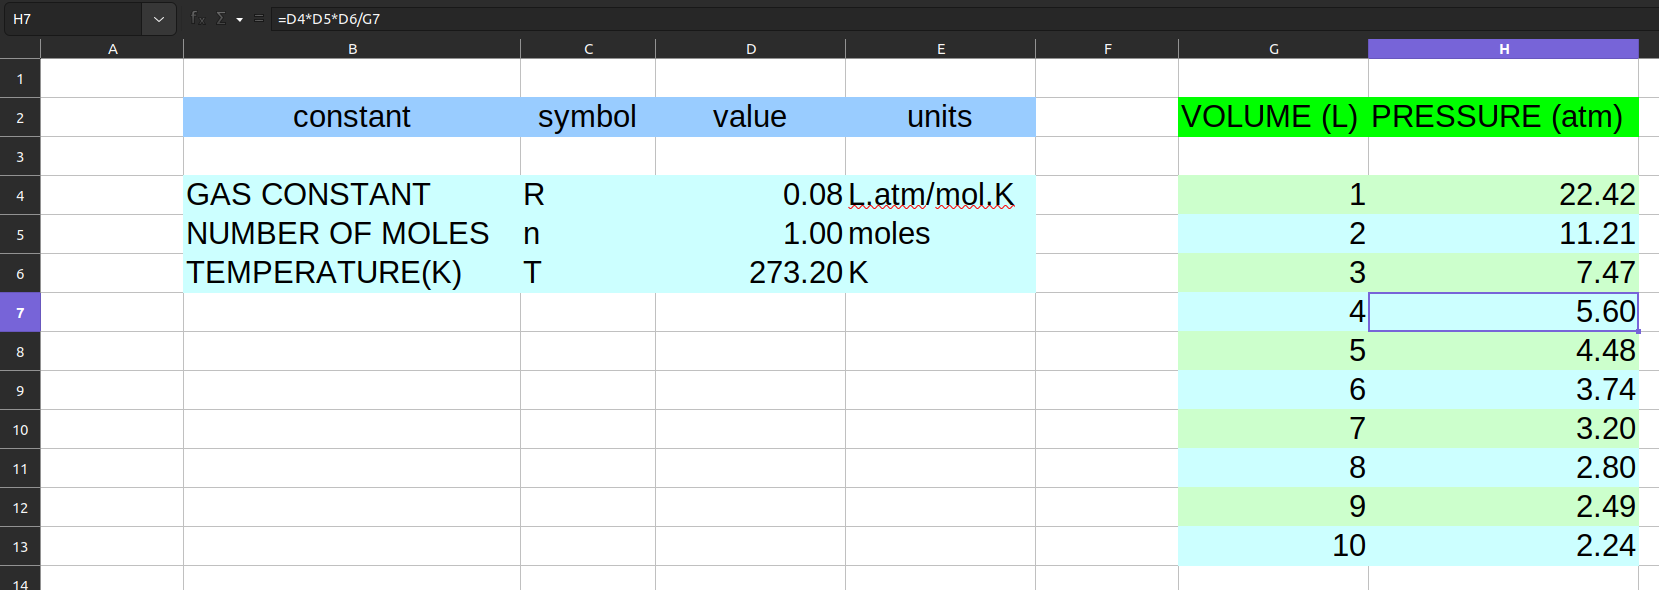
\includegraphics[scale=0.3]{Chapter4/volumePressure.png}
  \caption{Volume and pressure table}
  \label{fig:volumePressure}
\end{figure}

With formulas enabled, I obtained a spreadsheet as in \Cref{fig:volumePressureFormulas}.

\begin{figure}[h]
  \centering
  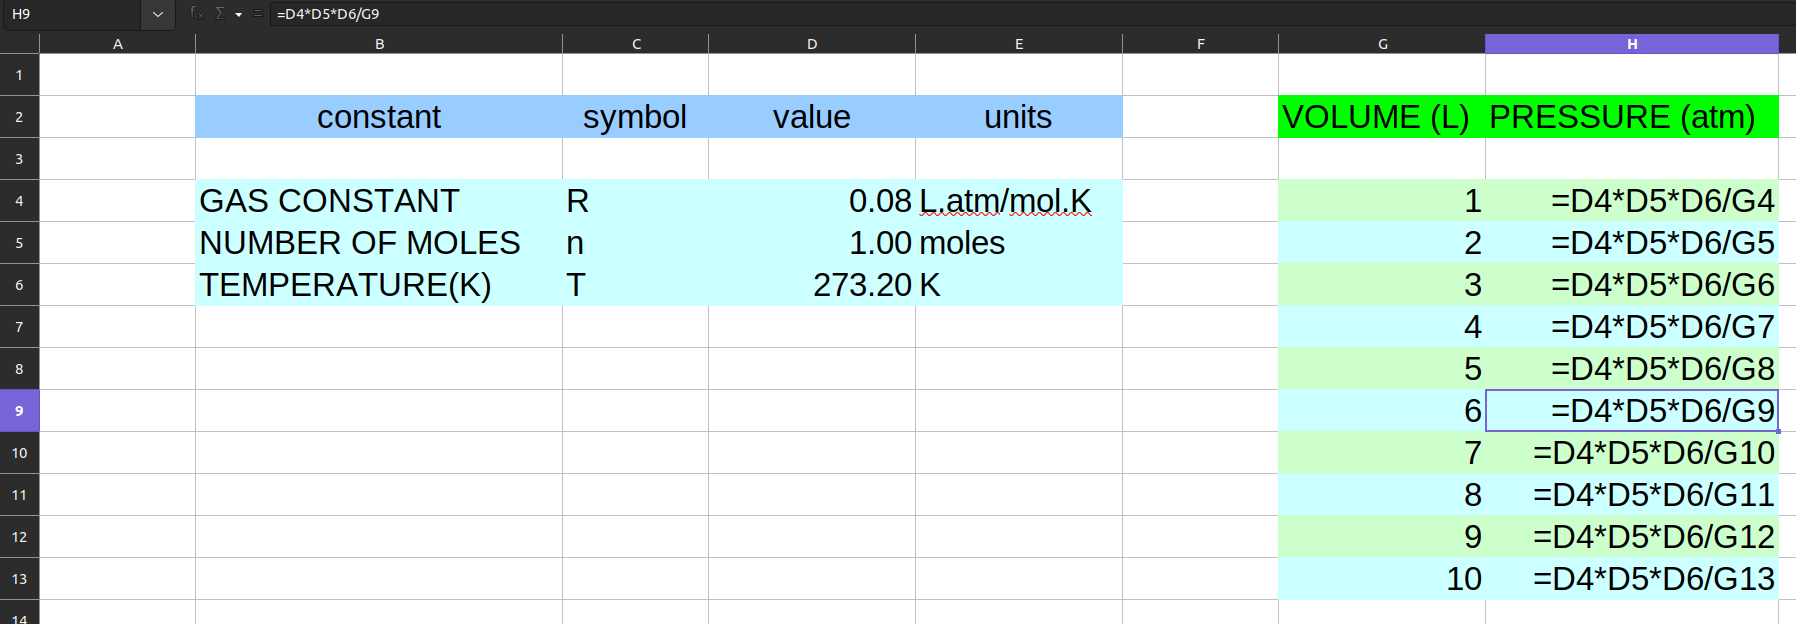
\includegraphics[scale=0.3]{Chapter4/volumePressureFormulas.png}
  \caption{Volume and pressure table with formulas enabled}
  \label{fig:volumePressureFormulas}
\end{figure}

\subsection{Language Extensions}

First, I enabled several language extensions.
\begin{itemize}
  \item \hs{DataKinds} allowed to promote values to type level.
  \item \hs{DuplicateRecordFields} allowed to use the same field names in multiple record data types.
  \item \hs{ImportQualifiedPost} allowed to use module imports of a specific form.
  \item \hs{OverloadedRecordDot} allowed to use the \hs{.} operator for accessing the record fields.
  \item \hs{RecordWildCards} allowed to omit the field names in records in certain cases.
\end{itemize}

\begin{listing}[!h]
  \begin{minted}{haskell}
{-# LANGUAGE DataKinds #-}
{-# LANGUAGE DuplicateRecordFields #-}
{-# LANGUAGE ImportQualifiedPost #-}
{-# LANGUAGE OverloadedRecordDot #-}
{-# LANGUAGE RecordWildCards #-}
{-# LANGUAGE TypeApplications #-}
\end{minted}
\caption{Language extensions}
\label{example3:extensions}
\end{listing}

\subsection{Imports}

Next, I imported the necessary Modules.

\begin{listing}[!h]
  \begin{minted}{haskell}
import Clerk
import Codec.Xlsx qualified as X
import Codec.Xlsx.Formatted qualified as X
import Lens.Micro ((%~), (&), (+~), (?~))
\end{minted}
\caption{Imports}
\label{example3:imports}
\end{listing}

\subsection{Tables}

The tables that I was going to construct were:

- A table per a constant's value (three of them)
- A volume and pressure table
- A constants' header
- A volume and pressure header

\subsubsection{Constants values}

\begin{figure}[h]
  \centering
  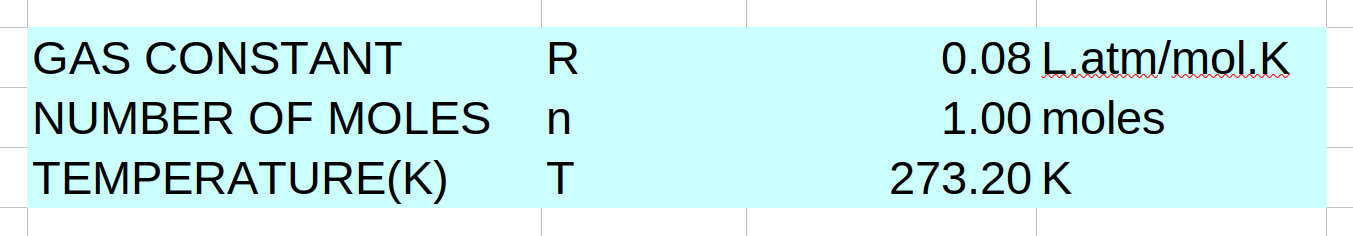
\includegraphics[scale=0.3]{Chapter4/constants.png}
  \caption{Constants values table}
  \label{fig:constants}
\end{figure}

In my case, each constant had the same type of the numeric value - `Double`.
That is why, I constructed a table with a single row per a constant and later placed the constants' tables under each other. I stored constant data in a record.

\begin{listing}[!h]
  \begin{minted}{haskell}
data ConstantData a = ConstantData
  { constantName :: String
  , constantSymbol :: String
  , constantValue :: a
  , constantUnits :: String
  }
\end{minted}
\caption{Constant data}
\label{example3:constantData}
\end{listing}

Next, I grouped the constants into a record. The parameter \texttt{f} may be an arbitrary type of kind \texttt{* -> *}.

\begin{listing}[!h]
  \begin{minted}{haskell}
data Constants f = Constants
  { gasConstant :: f Double
  , numberOfMoles :: f Double
  , temperature :: f Double
  }

type ConstantsInput = Constants ConstantData
\end{minted}
\caption{Constants}
\label{example3:constants}
\end{listing}

Following that, I recorded the constants data.

\begin{listing}[!h]
  \begin{minted}{haskell}
constants :: ConstantsInput
constants =
  Constants
    { gasConstant =
        ConstantData "GAS CONSTANT" "R" 0.08206 "L.atm/mol.K"
    , numberOfMoles =
        ConstantData "NUMBER OF MOLES" "n" 1 "moles"
    , temperature =
        ConstantData "TEMPERATURE(K)" "T" 273.2 "K"
    }
\end{minted}
\caption{Constant values}
\label{example3:constantValues}
\end{listing}

Now, I made a \texttt{RowI} for a constant input.
I used a \texttt{RowI} because this row requires the input type.
I would later use this row for each constant separately.

I got a pair of outputs:

- Top left cell of a constant table. That is, the cell with that constant name.
- The value of the constant.

Later, I would use these outputs to relate the positions of tables on a sheet.

Here, I used \texttt{lightBlue} from the \Cref{sec:styles}.

\begin{listing}[!h]
  \begin{minted}{haskell}
constant :: ToCellData a => RowI (ConstantData a) (Ref (), Ref a)
constant = do
  refTopLeft <- columnF lightBlue constantName
  columnF_ lightBlue constantSymbol
  refValue <- columnF (lightBlue .& with2decimalDigits) constantValue
  columnF_ lightBlue constantUnits
  return (refTopLeft, refValue)
\end{minted}
\caption{Language extensions}
\label{example3:constantCode}
\end{listing}

\subsubsection{Volume and pressure values}

\begin{figure}[h]
  \centering
  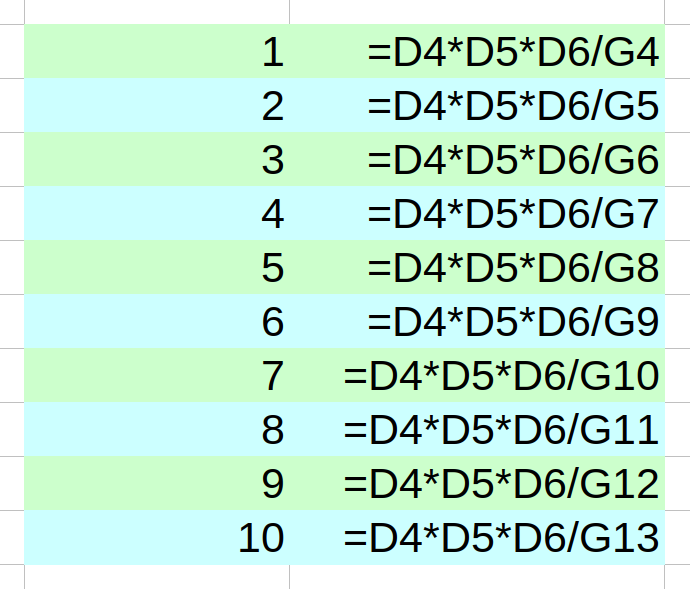
\includegraphics[scale=0.3]{Chapter4/valuesFormulas.png}
  \caption{Volume and pressure table with formulas enabled}
  \label{fig:valuesFormulas}
\end{figure}

I used the data and combined it with the constants to fill table \Cref{fig:valuesFormulas}

\begin{listing}[!h]
  \begin{minted}{haskell}
newtype Volume = Volume {volume :: Double}

volumeData :: [Volume]
volumeData = Volume <$> [1 .. 10]
\end{minted}
\caption{Language extensions}
\label{example3:volumeData}
\end{listing}

I made a helper type to pass the constants references in a structured way.

\begin{listing}[!h]
  \begin{minted}{haskell}
type ConstantsRefs = Constants Ref
\end{minted}
\caption{Constant references}
\label{example3:constantRefs}
\end{listing}

Next, I defined a function to produce a row for volume and pressure.

\begin{listing}[!h]
  \begin{minted}{haskell}
values :: ConstantsRefs -> RowI Volume ()
values Constants{..} = do
  refVolume <- columnF alternatingColors volume
  let pressure' = gasConstant .* numberOfMoles .* temperature ./ refVolume
  columnF_ (alternatingColors .& with2decimalDigits) (const pressure')
\end{minted}
\caption{Values}
\label{example3:valuesCode}
\end{listing}

\subsubsection{Constants' header}

\begin{figure}[h]
  \centering
  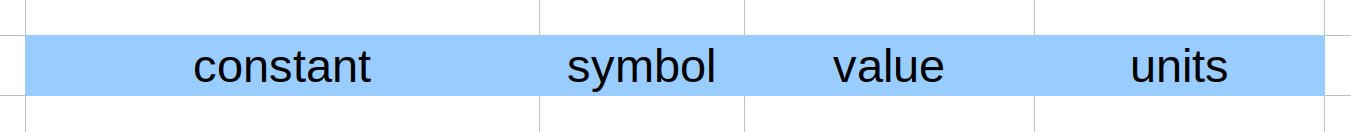
\includegraphics[scale=0.3]{Chapter4/constantsHeader.png}
  \caption{Constants header}
  \label{fig:constantsHeader}
\end{figure}

I did not use records here. Instead, I put the names of the columns straight into the `Row`. The outputs were the coordinates of the top left cell and the top right cell of this table.

\begin{listing}[!h]
  \begin{minted}{haskell}
constantsHeader :: Row (Ref (), Ref ())
constantsHeader = do
  let style :: FormatCell
      style = blue .& alignedCenter
  refTopLeft <- columnWF 20 style (const "constant")
  columnWF_ 8 style (const "symbol")
  columnF_ style (const "value")
  refTopRight <- columnWF 13 style (const "units")
  return (refTopLeft, refTopRight)
\end{minted}
\caption{Language extensions}
\label{example3:extensions}
\end{listing}

\subsubsection{Volume \& Pressure header}

\begin{figure}[h]
  \centering
  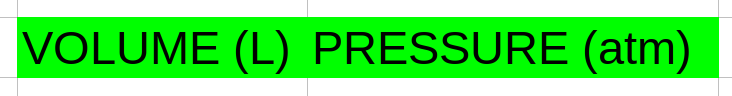
\includegraphics[scale=0.3]{Chapter4/valuesHeader.png}
  \caption{Header for the volume and pressure table}
  \label{fig:valuesHeader}
\end{figure}

For this header, I also put the names of columns straight into a row.

\begin{listing}[!h]
  \begin{minted}{haskell}
valuesHeader :: Row (Ref ())
valuesHeader = do
  refTopLeft <- columnWF 12 green (const "VOLUME (L)")
  columnWF_ 16 green (const "PRESSURE (atm)")
  return refTopLeft
\end{minted}
\caption{Language extensions}
\label{example3:extensions}
\end{listing}

\subsection{Sheet builder}

Finally, I combined all rows.

\begin{listing}[!h]
  \begin{minted}{haskell}
sheet :: Sheet ()
sheet = do
  start <- mkCoords 2 2
  (constantsHeaderTL, constantsHeaderTopRight) <- place start constantsHeader
  (gasTopLeft, gas) <- placeIn (constantsHeaderTL & row +~ 2) constants.gasConstant constant
  (nMolesTopLeft, nMoles) <- placeIn (gasTopLeft & row +~ 1) constants.numberOfMoles constant
  temperature <- snd <$> placeIn (nMolesTopLeft & row +~ 1) constants.temperature constant
  valuesHeaderTopLeft <- place (constantsHeaderTopRight & col +~ 2) valuesHeader
  placeIns (valuesHeaderTopLeft & row +~ 2) volumeData (values $ Constants gas nMoles temperature)
\end{minted}
\caption{Language extensions}
\label{example3:extensions}
\end{listing}

\subsection{Styles}
\label{sec:styles}

Below, I list the expressions used for sheet styling.

\begin{listing}[!h]
  \begin{minted}{haskell}
blue, lightBlue, green, lightGreen :: FormatCell
blue = mkColor (hex @"#FF99CCFF")
lightBlue = mkColor (hex @"#90CCFFFF")
green = mkColor (hex @"#FF00FF00")
lightGreen = mkColor (hex @"#90CCFFCC")

alternatingColors :: FormatCell
alternatingColors index = (if even index then lightGreen else lightBlue) index
\end{minted}
\caption{Language extensions}
\label{example3:extensions}
\end{listing}

Additionally, I composed an \texttt{FCTransform} for the number format.
Such a transform was used to accumulate cell formatting.

\begin{listing}[!h]
  \begin{minted}{haskell}
with2decimalDigits :: FCTransform
with2decimalDigits fcTransform =
  fcTransform & X.formattedFormat %~ X.formatNumberFormat ?~ X.StdNumberFormat X.Nf2Decimal
\end{minted}
\caption{Language extensions}
\label{example3:extensions}
\end{listing}

Finally, I made a transform for centering the cell contents.

\begin{listing}[!h]
  \begin{minted}{haskell}
alignedCenter :: FCTransform
alignedCenter = horizontalAlignment X.CellHorizontalAlignmentCenter
\end{minted}
\caption{Language extensions}
\label{example3:extensions}
\end{listing}
